\chapter{Introduction}\label{ch:intro}
	
	This master thesis was done at the University of Hildesheim in collaboration with Genie Enterprise Inc, Ludwigshafen. It investigates the use of image-to-image translation GAN for improving the character recognition of steel type plates/nameplates. This chapter introduces the problem statement with motivation, research questions, contributions and outline.

\section{Background}
 
 		Computer vision is the field of \gls{ai} that enables computers to see and process visual data. In simple words, it is a process of extracting information from images or videos. \gls{ocr} is a set of computer vision tasks that convert scanned documents and images into machine-readable text. Modern OCR algorithms can convert any type of text present in the image into digital information. The common applications of OCR are automatic license plate recognition, traffic sign recognition and extracting information from documents like cheque, invoice, passport, bank statement and business cards. The accuracy and success of OCR depend on the specific use cases. Every use case has its own challenges and requires different kinds of pre and post-processing of images. Our use case is to read text from the images of nameplates/steel type plates attached to power supply equipment.
\newline	
\begin{figure}
\centering
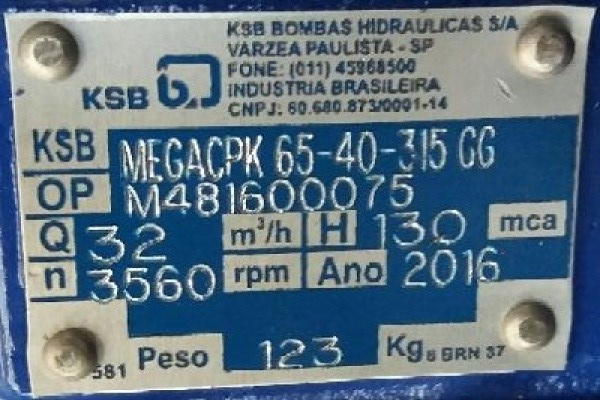
\includegraphics[width=3in,scale=1]{images/one.jpg}
\caption{ A sample steel type plate/nameplate image}
\label{fig:sampleimage}
\end{figure}
		Most electrical appliances such as motor come equipped with a nameplate/ steel type plate. The steel type plates that are attached to the motor contain a wealth of important information such as identification numbers, manufacturing year, \gls{hp}, \gls{rpm}, etc., This information describes their electrical properties needed to maintain and repair these devices. Figure \ref{fig:sampleimage} shows a sample steel type plate image in the dataset. These steel type plates differ in fonts, size, template and material used. The current practice is that the maintenance operator transcribes this information from the images of steel type plates for maintenance and repair. This manual approach is time-consuming and susceptible to errors but can be solved in real-time by the inference of a deep learning model. Hence we propose an automatic steel type plate recognition system.`	
\newline		

	
		Moreover, the steel type plate images are of poor contrast and include texts in corroded areas and difficult lighting conditions, such as reflections or shadows. Figure \ref{fig:rusted} shows the images of corroded steel type plates in different lighting conditions. These occlusions become problematic for automatic text extraction of the steel type plate images. Several related approaches exist to extract text from business cards, license plates and documents. But they usually consist of low noise or noise-free and do not need much intensive preprocessing of images for the extraction of texts. These assumptions cannot be guaranteed to be true in our case of weathered and rusted steel type plates since the stained areas contain a significant amount of text information. Hence most of the available OCR engines would fail in reading the steel type plates.
\newline	
	 
\begin{figure}
\centering
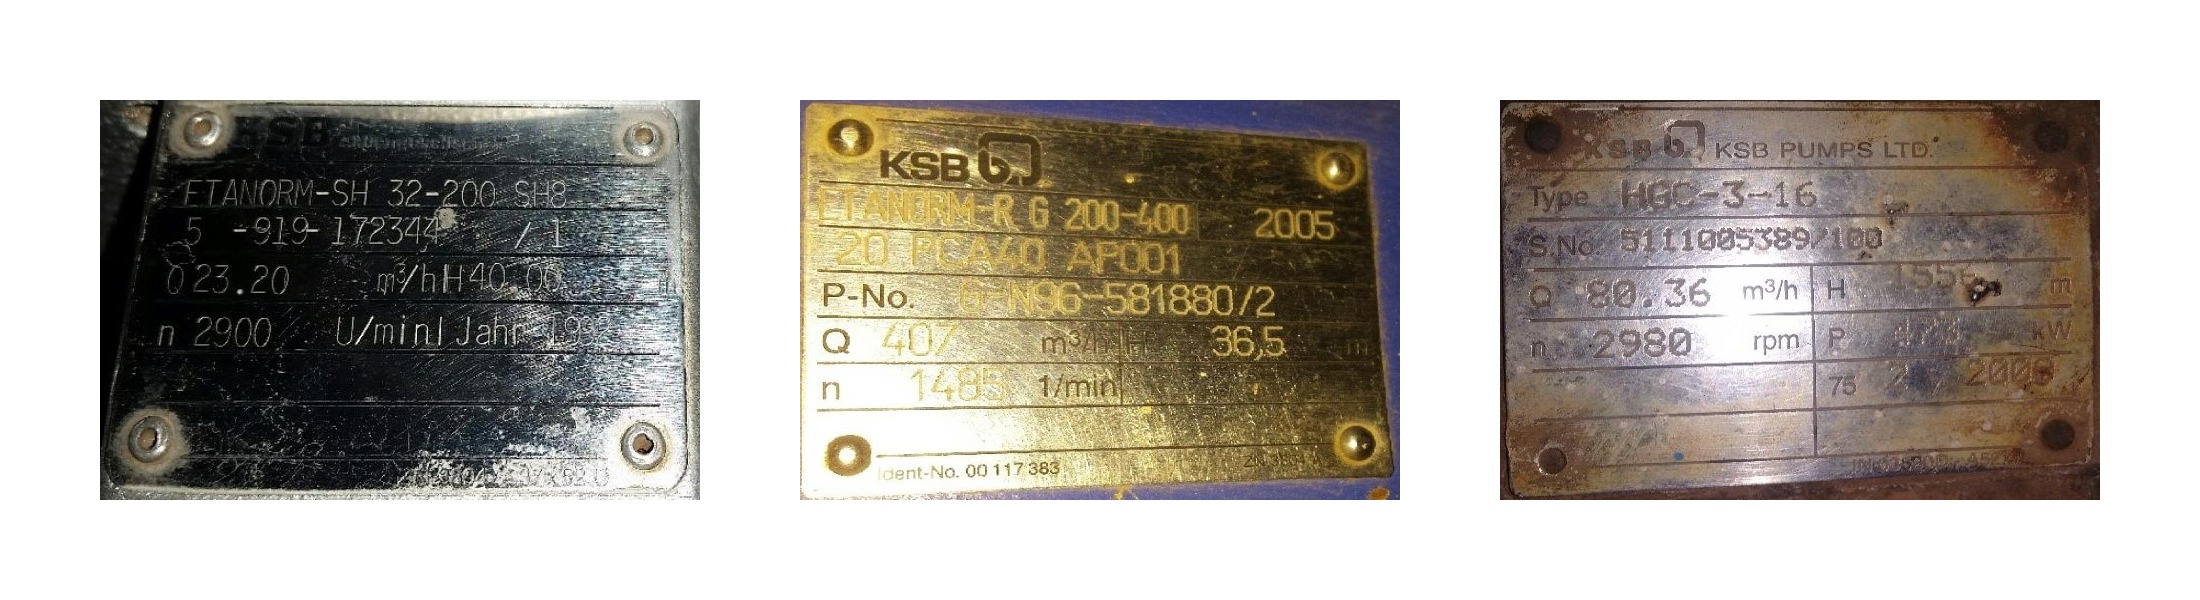
\includegraphics[width=5.5in]{images/corrode.jpg}
\caption{Weathered steel type plates under different lighting conditions}
\label{fig:rusted}
\end{figure}

		\gls{gan} is a generative model developed by Ian Goodfellow in 2014, which consists of two neural networks called generator and discriminator, competing against one another to improve their predictions \citep{goodfellow2014generative}. The image-to-image translation GANs are conditional adversarial networks that involve controlled modification of the image from a source domain to the target domain. Thus the automatic steel type plate recognition system consists of an image-to-image translation GAN for translating the noisy steel type plates into clear images and an OCR engine to extract text from the clear image. 

\section{Aim}
      
		The goal of the thesis is to find out if image-to-image translation GAN can be used as an image pre-processing method for steel type plate/nameplate images so that it improves the character recognition of OCR engines. Since the invention of conditional GAN, several works on image-to-image translation have been proposed. We investigate three kinds of image-to-image translation GAN models that were chosen based on their different learning approaches in order to select the best model for optimizing the steel type plate images: i) \cite{isola2017image} proposed pix2pix GAN that works by learning the mapping between the source domain and the target domain using paired dataset. ii) \cite{CycleGAN2017} proposed CycleGAN is an unsupervised way of training image-to-image translation models. It does not require a paired dataset for training instead uses an unordered collection of images from two different domains. iii)  \cite{stoller2019training} proposed FactorGAN trains image-to-image translation models when data points are incomplete in semi-supervised fashion. Thus, the proposed framework uses the best generator model out of the above three GANs to translate the noisy image to a clean image and then extract text from these optimized images through an OCR engine.
		
\section{Research questions}

In order to achieve the aim, this thesis will answer the following questions:
\begin{enumerate}
\item Can an image-to-image translation GAN be used to improve the accuracy of character recognition for the images of weathered steel type plates?
\item Can the findings of \citeauthor{CycleGAN2017} and \citeauthor{stoller2019training} be used to make up for the few image pairs in the steel type plate dataset?
\item How to evaluate the three different image-to-image translation GAN models under the scope of the thesis and choose the optimal model for the proposed steel type plate recognition system?
\item How good is the proposed GAN engine compared to a commercial OCR tool like Google Vision? How can the performance of the overall framework be measured?	
\end{enumerate}

\section{Contributions}  	
	This thesis examines the in-depth analysis of using generative models to improve the text detection and character recognition in the context of images of steel type plates/nameplates attached to the electrical equipment.
\newline
	
	A dataset of steel type plate/nameplate images was created with approximately 500 images crawled from google image search using python scripts. Then labels were manually created for those images which are explained briefly in Chapter \ref{ch:exp}. A unique approach is used to create synthetic data close to real image distribution to mitigate the problem of fewer image pairs in the dataset. The synthetic dataset consists of images with its corresponding output pair. Then the use of three kinds of image-to-image translation GAN was investigated to improve the robustness of the OCR engine against the images with adverse lighting and occlusions. The hyperparameters were tuned to get an optimal combination and the experiments were conducted to select the best GAN generator model for integration with the OCR engine.
\newline
	
	Different evaluation metrics for GAN like \gls{ssim}, \gls{fid} score and \gls{mse} were explored. The GAN model is evaluated using both qualitative and quantitative metrics. The proposed OCR engine was built by integrating a CRAFT based text detection model and a text recognition model. In order to evaluate the accuracy of the proposed OCR engine, it is compared with one of the benchmark OCR engines like Google Vision OCR. Finally, both the OCR engines are evaluated with original images as well as GAN translated images. The results were tabulated and analyzed using bar graphs to get a better understanding which is briefly discussed in Chapter \ref{ch:results}.
 
\section{Thesis outline}

		The rest of the report is organized as follows:
Chapter \ref{ch:related} discusses the literature review and background that is relevant to understand the thesis. Deep learning sets the foundation throughout the thesis and thus a general introduction to neural networks, generative models and OCR models is provided in this chapter. Chapter \ref{ch:method} introduces the proposed framework, where we discuss the overall architecture and training procedure in detail for each of the components; Chapter \ref{ch:exp} focuses on the dataset collection and description with insights. Besides, this chapter discusses briefly the creation of labels and how the synthetic dataset was created. Chapter \ref{ch:results} presents the results obtained from the experiments both quantitatively and qualitatively along with the experimental setup. A brief discussion on the result is provided with several insights and visual samples of GAN generated images. Finally, Chapter \ref{ch:conclusion} concludes the thesis research with remarks and provides possibilities for future research directions.


